\section{Neural Networks (NNs)}\label{sec:neural-networks-(nns)}

As previously mentioned in the Preface, an artificial neural network (ANN or NN) is a mathematical model for data processing, initially inspired by the structure of the brain.
Therefore, a brief overview of how a brain functions is presented next.

\subsection{Neurons in the Brain}\label{subsec:neurons-in-the-brain}
Inside the brain, around 86 million neurons\footcite{caruso_23} form connections to each other through which they activate other neurons with electric and chemical signals.
In a neuron, the signals of connected neurons add up and when they reach a certain threshold, the neuron is activated and fires a new signal to its own connections\footcite{Newman_23}.
The neuron then resets after a certain amount of cooldown time.
\\
With this web of neurons inside the brain, animals can process the information from nerve signals from the body and output them again as nerve signals instructing the body.

\subsection{Feed Forward Neural Networks (FNNs)}\label{subsec:feed-forward-neural-networks-(fnns)}
So how can these ideas about neural networks learned from the biology of a brain be applied to a program that runs on a computer?
The first step is to simplify the chaos of neurons in the brain and organize them into layers of neurons.
These layers consist of an input layer, an output layer and optional so-called hidden layers in between.
As a next step, the neurons in each layer are connected to those in subsequent layers, typically limited to connections with the nearest layer.\footcite{Hardesty2017}
\\
Now, the structure of a neural network looks something like this:
\begin{figure}[H]
    \centering
    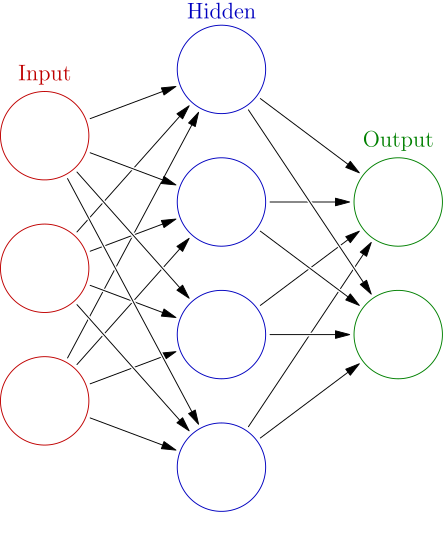
\includegraphics[width=0.25\textwidth]{nn_simple_1}~\caption{A simple Feed Forward Neural Network (FNN) with three layers: Input, Hidden and Output.\footnote{\cite{nn_simple_img_1}}}
    \label{fig:nn_simple_1}
\end{figure}

To describe the specific structure of a NN, the term topology is used\@.
\begin{mydef}{Neural Network Topology}
    The topology of a neural network is its distinct arrangement of neurons, layers and the connections between the neurons.\footcite{Miikkulainen2010}
    \label{definition:Topology}
\end{mydef}
For the neural network to perform functions, a weight needs to be assigned.
This weight value ranges from -1 to 1 and can be thought of as the strength of a connection between neurons.
\\
In terms of computer science, this structure now resembles a directed, weighted graph, which is why the neurons are called nodes and their connections edges.
\begin{mydef}{Nodes/Edges}
    In a neural network, a node receives, computes and sends information, whereas an edge forms the connections between nodes to exchange information.\footcite{Sanchez-Lengeling2021}
    \label{definition:Nodes-Edges}
\end{mydef}
\\ \\
The computation process of information by a neural network can be illustrated through the example of a computer vision NN that recognizes digits in a black-and-white image.
As a first step, the input is encoded into values that correspond to the nodes of the input layer.
In the example of a computer vision NN, the brightness values of the single pixels might directly represent the nodes of the input layer.
\\
Then, the algorithm iterates through all input nodes to identify its connected edges.
For each of these edges it multiplies its weight by the value of the input node and adds the result to the node on the receiving end.
\\
After iterating through all the nodes of one layer, it moves to the next layer.
At this point, the value of the nodes in the current layer is the sum accumulated by the values of all connected nodes multiplied by the weight of that connection:
\begin{equation}
    v_x = \sum_{i=0}^{N}v_i * w_i\label{eq:sum_connected_nodes}
\end{equation}
Where:
\textit{
    \begin{itemize}
        \item $v_x$ is the value of the current node
        \item N is the number of connected nodes
        \item $v_i$ is the value of the connected node i
        \item $w_i$ is the weight of the edge connecting the current node to node i
    \end{itemize}
}

Additionally, some algorithms add a bias value $r_x$ ranging from -1 to 1 onto the value of the nodes.\footcite{IBMNeuralNetworks}
Finally, an activation function\footcite{Baheti2021} $\sigma(x)$ is applied to the value of the nodes to fit the value of the node inside a preferred range.
This activation function can also be thought of as the threshold of stimulation for a neuron to fire.
Two examples for activation functions are:
\begin{itemize}
    \item Sigmoid Function: $\sigma(x) = \frac{1}{1 + e^{-x}}$
    \item Rectified Linear Unit (ReLU): $\sigma(x) = \max{0, x}$
\end{itemize}
Plot of the activation functions:
\\ \\
\begin{center}
    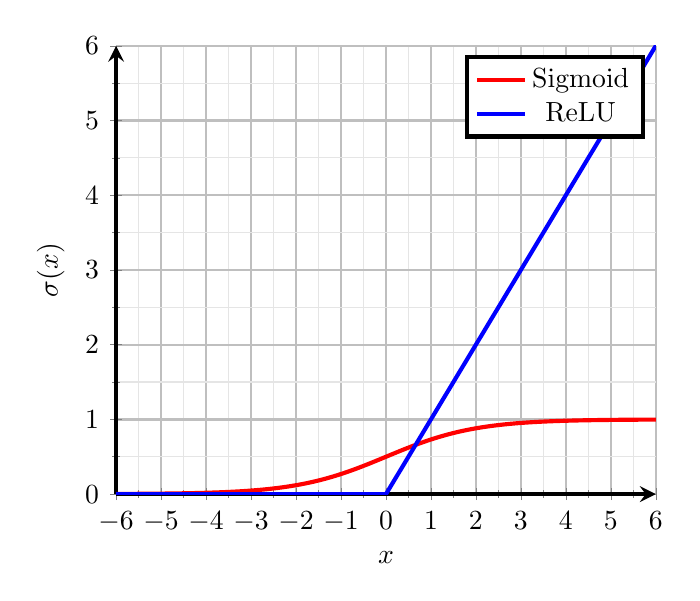
\begin{tikzpicture}
        \begin{axis}
            [
            xmin=-6,
            xmax=6,
            ymin=0,
            ymax=6,
            ytick distance = 1,
            xtick distance = 1,
            minor tick num=1,
            axis lines = left,
            line width = 1.5pt,
            grid=both,
            major grid style={line width=0.8pt,draw=gray!50},
            minor grid style={line width=0.4pt,draw=gray!20},
            xlabel = \(x\),
            ylabel = {\(\sigma(x)\)}
            ]
            % First plot (Sigmoid)
            \addplot[
                domain=-10:10,
                color=red,
                samples=1000,
            ]{1/(1 + e^-x)};

            % Second plot (ReLU)
            \addplot[
                domain=-10:10,
                color=blue,
                samples=1000,
            ]{max(0,x)};

            % Define the legend after all plots have been added


            \legend{Sigmoid, ReLU}

        \end{axis}
    \end{tikzpicture}
\end{center}

~\\
The complete function for the value of one node is therefore:
\begin{equation}
    v_x = \sigma\left(\sum_{i=0}^{N}v_i * w_i + r_x\right)\label{eq:value_node}
\end{equation}
Where (additionally to equation~\ref{eq:sum_connected_nodes}):
\textit{
    \begin{itemize}
        \item $r_x$ is the bias of the node
        \item $\sigma$ is the activation function
    \end{itemize}
}

Now this value $v_x$ is again sent through its connections to nodes in the upcoming layers.
After iterating through all the nodes and layers of the neural network (NN), the process reaches the final layer of the NN, where the computed output can be read out.
This output is encoded in node values, as was done with the input, and therefore requires decoding to obtain the final result.
In the example of a digit-detecting NN, 10 output nodes could be used, each representing one digit.
The result could then be decoded by identifying the output node with the highest value as the result.
This kind of output encoding, where all possible results are assigned their own node, is referred to as one-hot output encoding\footcite{Brownlee2020}.
With one-hot output encoding, the values of the output nodes can be interpreted as a the neural networks certainty for a specific result to be correct.

\subsection{Remark: Functioning of NNs}\label{subsec:remark-about-the-funtioning-of-nns}
Having established how a neural network operates, it is important to understand why this type of algorithm is considered revolutionary in the field of computer science.
\\ \\
An algorithm processes an input with a set of functions applied in a certain order to calculate an output.
Traditionally, a computer algorithm gets programmed with the help of mathematical operations, logic functions, loops, system functions, and data structures, which are then converted into binary code for the processor.
Of course, this also applies in the context of NNs.
However, there is also a third layer of abstraction on top, which simulates the functioning of a brain with neurons.
Since the traditional algorithm only enables the neurons of a NN, the third neuron-based layer is what computes the actual function of the NN. Therefore, NNs resemble more the functioning of a brain than a traditional algorithm.
\\
\begin{figure}[H]
    \centering
    % Subfigure 1: Traditional Algorithm
    \begin{subfigure}[t]{0.45\textwidth}
        \centering
        \begin{tikzpicture}[node distance=2cm]
            % Left pile (Traditional Algorithm - 2 layers)
            \node (trad_top) [level, fill=red!40] {
                Deterministic Algorithm\\
                \small{(Operations, logic, loops, etc.)}
            };
            \node (trad_bottom) [level, below of=trad_top] {
                Binary Code\\
                \small{(Processor instructions)}
            };

            % Label
            %\node[above=0.5cm of trad_top, font=\Large] {Traditional Algorithm (2 layers)};

            % Arrow
            \draw[->, thick] (trad_top.south) -- (trad_bottom.north);
        \end{tikzpicture}
        \caption{Traditional Algorithm (2 layers)}
    \end{subfigure}
    \hfill
    % Subfigure 2: Neural Network
    \begin{subfigure}[t]{0.45\textwidth}
        \centering
        \begin{tikzpicture}[node distance=2cm]
            % Right pile (Neural Network - 3 layers)
            \node (nn_top) [level, fill=red!40] {
                Neuron Activation\\
                \small{(Simulated neurons, brain-like structure)}
            };
            \node (nn_middle) [level, below of=nn_top] {
                Deterministic Algorithm\\
                \small{(Enables the functioning of NNs)}
            };
            \node (nn_bottom) [level, below of=nn_middle] {
                Binary Code\\
                \small{(Processor instructions)}
            };

            % Label
            %\node[above=0.5cm of nn_top, font=\Large] {Neural Network (3 layers)};

            % Arrows
            \draw[->, thick] (nn_top.south) -- (nn_middle.north);
            \draw[->, thick] (nn_middle.south) -- (nn_bottom.north);
        \end{tikzpicture}
        \caption{Neural Network (3 layers)}
    \end{subfigure}
    \caption{The Neural Network algorithm replaces the function of data-processing (colored in red) that is traditionally done by a deterministic algorithm.}\label{fig:figure}
\end{figure}

\\
This difference has implications for the functioning of an NN: Traditional algorithms represent actual mathematical calculations and are therefore deterministic.
With NNs, the algorithm is based on different parameters for nodes and edges, which make it an unpredictable black box.
In the top layer of abstraction, there are no concrete functions but only neuron activation that approximates a function instead.
This means it is hard to prove a neural network to always be accurate and is also the reason why the result of NNs is often called its prediction. \footcite{springer_blackbox}%nature_blackbox,

\begin{mydef}{NN Prediction}
    The output of a neural network is referred to as its prediction for a given input.\footcite{Warudkar2020}
\end{mydef}

\subsection{An Example of NN learning: Backpropagation}\label{subsec:an-example-of-nn-learning:-backpropagation}
It has already been established how a neural network with specific parameters generates a prediction for a given input.
This however raises the question: how can parameters encoding the structure, weights, and biases of the neural network be determined?
The solution lies in using machine learning, which trains the model to perform a specific task using training data.
\begin{mydef}{Machine Learning}
    Machine learning (ML) is a branch of artificial intelligence that focuses on optimizing artificially intelligent models to solve a given problem.\footcite{IBM_Machine_Learning}
\end{mydef}
One machine learning algorithm for NNs is called backpropagation, which is one of the simplest and most efficient methods to train a NN.\footcite{Al-Masri2024}
Backpropagation works using a training and test set containing labeled data for a problem.
\begin{mydef}{(Un)labeled Data}
    Labeled data for a machine learning problem is a set of data with sample problems and the respective solutions.
    Unlabeled data instead only contains the sample problems.\footcite{IBM_Data_Labeling}
\end{mydef}
The machine learning process of backpropagation begins with a neural network that has a fixed topology and random weights and biases.
First, the NN is given the training problems for which it will generate random predictions.
These random predictions are then refined using the sample solutions.
This is done by looping back through the NN from the output layer to the input layer, always adjusting the weights and biases in a way that the NN would finally make the right prediction for this problem.
However, the NN shouldn't be adapted only to a single problem but make accurate predictions for the whole training set and unknown problems.
To therefore prevent overcorrecting a NN for single problems, a learning rate significantly smaller than 1 is applied to the corrections.
\\ \\
The NN is trained on the whole training set for many generations, until the NN starts to make accurate predictions for all problems.
To evaluate the performance on unknown problems, a separate test set, which the NN hasn't been trained on, can be used.


\section{Evolutionary Computation (EC)}\label{sec:evolutionary-computation-(ec)-&-genetic-algorithms-(gas)}
The focus now shifts to the machine learning technique this thesis focuses on.
Once again, nature serves as inspiration:
\begin{mydef}{Evolutionary Computation}
    Evolutionary Computation (EC) is an Algorithm that optimizes a set of parameters for a problem with the help of natural selection.\footcite{virtusa2024}
\end{mydef}
Evolutionary computation (EC) is often employed in situations where the optimal parameters for a function cannot be directly calculated, but the performance of a given parameter set can be evaluated.
One example scenario involves a large dataset of points representing an unknown polynomial function with added noise and outliers.
To determine the parameters of the underlying polynomial, EC can be utilized to identify the best-fitting parameters.
The following shows how EC achieves this optimization.
\\ \\
The process starts with an initial population of agents with random parameter sets.
EC then repeats following steps, forming a new generation of the population in each iteration\footcite{Sathyabama20}:
\begin{itemize}
    \item \textbf{Fitness evaluation:} First, EC assesses the performance of each agent, defined by its parameters, in the given problem.
    This performance is referred to as the agent's fitness, which can be evaluated either objectively through a cost function or relatively with a competition between agents.
    In the given example, the cost function might check the prediction of the NN for the given data points, calculate the absolute differences between the prediction and the values of the data points, and use the total sum of these differences as the cost.
    \item \textbf{Selection:} As a next step, the agents that performed well are selected to be part of the next generation.
    \item \textbf{Reproduction:} The selected agents are then replicated by directly copying their parameters (non-mating) or by merging parameters from different agents (crossover).
    \item \textbf{Mutation:} In each new generation, the parameters of the agents are mutated, either by completely replacing certain parameters with new random parameters or by shifting the existing parameters by a random value.
\end{itemize}
After a certain number of generations, the EC algorithm will have found best performing set of parameters for a given problem.

\subsection{Gradient Descent}\label{subsec:gradient-descent}
As established in the previous section, EC begins with an initial population of agents with a random set of parameters.
The fitness of these agents is determined using a cost function.
Agents with relatively low cost (or high fitness) survive the round and are replicated, mutated and again selected by cost.
\\ \\
This whole process strongly resembles a ball rolling down a hill in some terrain.
At any given point on the terrain, the ball moves in the direction of the steepest descent (ignoring the inertia of the ball).
Applying this analogy to EC, the parameters for a function can be imagined as the horizontal coordinates for the ball meanwhile the cost of these parameters correspond to the height at that location.
Mutations produce parameter sets that are close to the original, resembling neighboring points on the terrain.
As the ball rolls down to the lowest neighboring point in any step, EC again chooses the set of parameters with the lowest cost every cycle.
This is why the machine learning process is referred to as gradient descent, as the algorithm evaluates all neighboring points and then follows the direction with the lowest cost and therefore steepest gradient\footcite{ibm2024}.

\subsection{Initial Position \& Local Minima}\label{subsec:initial-position-&-local-minima}
The ball analogy provides insights into the functioning of the EC learning process, which can be understood by visualizing a hill with each a shallow and a deep valley next to it.
Depending on which side of the hill the ball is placed in the beginning, it will roll in a different direction and end up in either of the two valleys, which have different heights.
Therefore, following things can be derived:
\begin{itemize}
    \item (Minor) differences in the starting position can result in large differences in the end position and the respective cost.
    \item Once a point with no downwards gradient is reached, innovation halts for that agent, even if there is a point with lower cost somewhere else.
    Such points are called local minima.
\end{itemize}

\begin{figure}[H] % Wrap in figure environment

    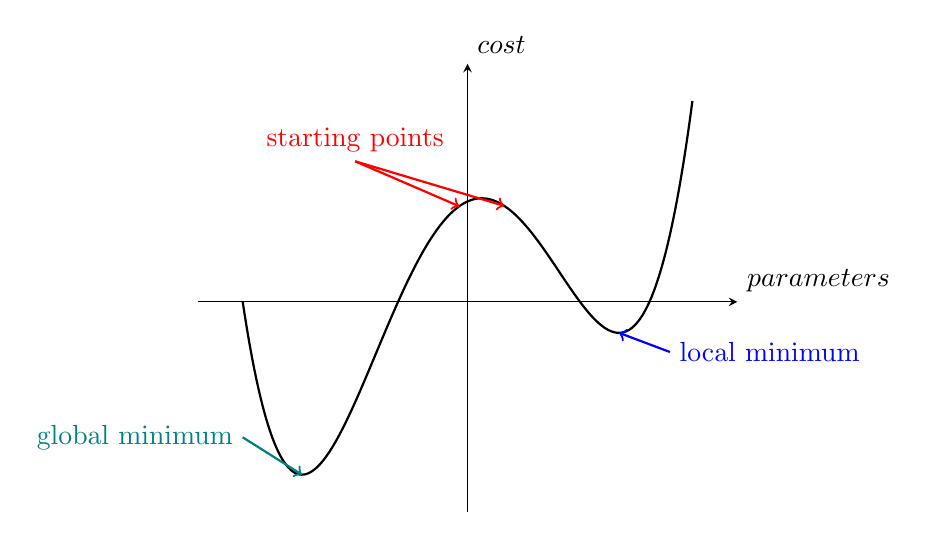
\begin{tikzpicture}
        \begin{axis}
            [
            axis lines=middle,
            xlabel={$parameters$},
            ylabel={$cost$},
            domain=-2:2,
            samples=200,
            enlargelimits=0.1,
            ticks=none,
            clip=false,  % Allow labels/arrows outside the plot area
            label style={anchor=south west},
            ]
            % Plot the function
            \addplot[thick,black] {x^4 -4*x^2 + x + 2};

            % Coordinates of extrema:
            \coordinate (starting1) at (axis cs:-0.074,1.9041);
            \coordinate (starting2) at (axis cs:0.326,1.9122);
            \coordinate (MinLeft) at (axis cs:-1.473,-3.444);
            \coordinate (MinRight)at (axis cs:1.347,-0.618);

            % Starting points (in the displayed range, the highest stationary point)
            % Adjust arrow start and label position so they are not cut off.
            \draw[->,red,thick] (axis cs:-1,2.8) -- (starting1);
            \draw[->,red,thick] (axis cs:-1,2.8) -- (starting2);
            \node[red,above] at (axis cs:-1,2.8) {starting points};

            % Local minimum (right)
            \draw[->,blue,thick] (axis cs:1.8,-1) -- (MinRight);
            \node[blue,right] at (axis cs:1.8,-1) {local minimum};

            % Global minimum (left)
            \draw[->,teal,thick] (axis cs:-2,-2.7) -- (MinLeft);
            \node[teal,left] at (axis cs:-2,-2.7) {global minimum};

        \end{axis}
    \end{tikzpicture}
    \caption{The effect of the starting position on the final cost of the parameters with gradient descent.}
    \label{fig:gradient_descent}
\end{figure}
\begin{mydef}{Local Minimum}
    A local minimum is a point with minimal cost compared to its neighboring area and is therefore a halting point for gradient descent.\footcite{ayoosh2024}
\end{mydef}
The impact of starting position and local minima often pose a large problem for EC applications.
Strategies to reduce the impact of such are therefore crucial for the algorithms success.


\section{Evolutionary Neural Networks (ENNs)}\label{sec:evolutionary-neural-networks-(enns)}
After having covered all the basics about neural networks and evolutionary computation, the two concepts are finally combined to create the algorithm this thesis focuses on.
\begin{mydef}{Evolutionary Neural Networks}
    Evolutionary neural networks (ENNs) are neural networks that use an evolutionary algorithm called neuroevolution to optimize for its parameters for the NNs weights/biases and its topology.\footcite{enn22, neuroevolution19}
\end{mydef}
ENNs are useful for complex machine learning problems and also work for unlabeled training data as long as there is a fitness function.
In the context of neural networks, evolutionary computation can be applied as follows:
\\
The parameters encoded by ENNs represent the weights, biases, nodes, and edges of a neural network.
ENNs still follow the same core process of evolutionary computation:
They start with a random population of NNs that are evaluated and selected based on a fitness function.
The selected NNs are replicated (with crossover or non-mating) and finally mutated in following ways:
\begin{enumerate}
    \item \textbf{Change weights/biases:} A new random value is set for the weight or bias of a random existing edge or node.
    \item \textbf{Shift weights/biases:} The value for an existing weight or bias of a random existing edge or node is altered by a random change but is kept close to the old value.
    \item \textbf{Add edges:} A new edge is added between two random, previously unconnected nodes.
    \item \textbf{Add nodes:} A new node is added in between of a random existing edge.
    The old edge is removed and two new edges with random weights are added between the new node and the two other nodes each.
    \item \textbf{Remove nodes/edges:} A random node or edge is removed in a way that doesn't cut off the input from the output layer.
\end{{enumerate}}


\section{The NEAT-Approach}\label{sec:the-neat-approach}
As already stated in the thesis statement(\ref{sec:thesis-statement}), neuroevolution of augmenting topologies is an ENN machine learning algorithm developed by Kenneth O. Stanley and Risto Miikkulainen in 2002\footcite[p.105-106]{Neat_02}.
NEAT evolves the topology, weights and biases of NNs at the same time, which makes it particularly suitable for tasks where the optimal network architecture is not yet known.
One of its key innovations is that the initial population begins with NNs of lowest complexity and the NNs only increase topological complexity as it is useful for the problem.
In specific, the NEAT algorithm starts with NNs that only have the nodes of the input layer connected to the nodes of the output layer.
This design aims to produce more efficient neural networks by only increasing complexity when it leads to improved performance.
The NEAT algorithm therefore only needs the mutations 1. to 4. shown in the last section(\ref{sec:evolutionary-neural-networks-(enns)}) and doesn't need to remove complexity (mutation 5.) as it is already minimal.


\section{Games}\label{sec:games}
The following section offers a brief overview of the games on which the ENNs will be trained.

\subsection{Simple Nim}\label{subsec:simple-nim}
This game is a simplified version of Nim, where two players take turns removing an arbitrary amount of matches from a single stack with some number of matches.
The player who removes the last match loses.
Therefore, the winning strategy simply is to remove all matches from the stack but one, forcing the opponent to remove the last match and therefore making them lose.

\subsection{Nim}\label{subsec:nim}
This game works similarly to Simple Nim with the difference that there are multiple stacks with matches.
Now, the player who removes the last match from the last unemptied stack loses.
The winning strategy for Nim involves a binary representation of the game state\footcite{rosenbloom2003} and is therefore mathematically much more complex, which forces the ENNs to learn more sophisticated strategies.


\section{Related Work}\label{sec:related-work}
The field of AI research in ENNs is largely studied and is often linked to games.
The following table provides some examples of ENN models that have been tested on games:

\footnotesize
\begin{center}
    \hspace*{-2cm}\begin{tabular}{|| l l l l l ||}
                      \hline
                      \makecell{\textbf{Author(s) \& Year}} &
                      \makecell{\textbf{Model}} &
                      \makecell{\textbf{Game/Benchmark}} &
                      \makecell{\textbf{Computation}} &
                      \makecell{\textbf{Accuracy}} \\
                      \hline\hline
                      \makecell{\cite{Neat_02}} &
                      \makecell{NEAT} &
                      \makecell{Double Pole Balancing \\With Velocities} &
                      \makecell{3600 \\evaluations} &
                      \makecell{100\%} \\
                      \hline
                      \makecell{\cite{dama_22}} &
                      \makecell{NEAT} &
                      \makecell{Dama} &
                      \makecell{$>$5000 \\generations} &
                      \makecell{81.25\%\\(wins against humans)} \\
                      \hline
                      \makecell{\cite{go_98}} &
                      \makecell{SANE} &
                      \makecell{Go} &
                      \makecell{260 \\generations} &
                      \makecell{$>$75\%\\(vs Wally, 9$\times$9 board)} \\
                      \hline
                      \makecell{\cite{capture_02}} &
                      \makecell{Custom \\ENN} &
                      \makecell{Capture Game\\(subgame of Go)} &
                      \makecell{$>$100 \\generations\\(distributed)} &
                      \makecell{No significant \\progress yet} \\
                      \hline
                      \makecell{\cite{backgammon_07}} &
                      \makecell{Genetic \\ENN} &
                      \makecell{Backgammon} &
                      \makecell{256 pop,\\100–200 \\generations} &
                      \makecell{62.4\%\\(vs Pubeval)} \\
                      \hline
    \end{tabular}\hspace*{-2cm}
\end{center}
\normalsize
Note:
Although the amount of fitness evaluations is a more accurate representation of computation load than the amount of generations, in many cases the amount of fitness evaluations isn't indicated and cannot be derived.